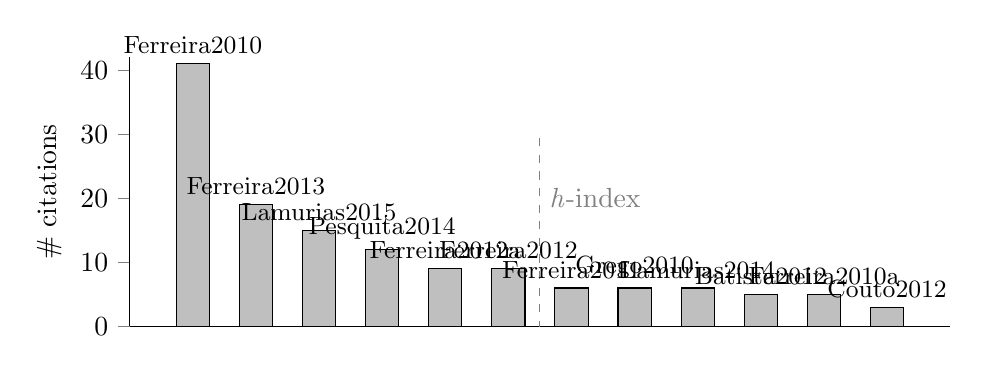
\begin{tikzpicture}
\begin{axis}[
    width=12cm,height=5cm,
    xmin=0,xmax=13,xminorticks=false,xmajorticks=false,
    ymin=0,ymax=42,
    ytick align=outside,
    axis x line*=bottom,axis y line*=left,
    tick label style={/pgf/number format/assume math mode=true},
    ylabel={\# citations},
    % enlargelimits=0.15,
    ybar,
    bar width=12pt,
]
\addplot[
    fill=lightgray,
    nodes near coords,
    point meta=explicit symbolic,
    every node near coord/.append style={font=\small}
]
    coordinates{
        (1,41) [\autocite{Ferreira2010}]
        (2,19) [\autocite{Ferreira2013}]
        (3,15) [\autocite{Lamurias2015}]
        (4,12) [\autocite{Pesquita2014}]
        (5,9)  [\autocite{Ferreira2012a}]
        (6,9)  [\autocite{Ferreira2012}]
        (7,6)  [\autocite{Ferreira2011}]
        (8,6)  [\autocite{Grego2010}]
        (9,6)  [\autocite{Lamurias2014}]
        (10,5) [\autocite{Batista2012}]
        (11,5) [\autocite{Ferreira2010a}]
        (12,3) [\autocite{Couto2012}]
        % (13,2) [\autocite{Tavares2010}]
        % (14,1) [\autocite{Ferreira2016}]
        % (15,1) [\autocite{Ferreira2014}]
        % (16,1) [\autocite{Lamurias2014a}]
        % (17,1) [\autocite{Ferreira2013a}]
    };
\addplot[gray,line legend,dashed,sharp plot,update limits=false]
    coordinates {
        (6.5,-3)
        (6.5,30)
    }
    node[right] at (6.5,20) {\textit{h}-index};

\end{axis}
\end{tikzpicture}
